\documentclass[10pt,a4paper]{article}
\usepackage{graphicx,float}

\title{\LARGE
    Project Phase 1: A Detailed Analysis of SUPERCOP on the Dragonboard APQ8060.
}

\author{\large
{\bf Kevin Burns, Robert Lyerly, Reese Moore, Philip Kobezak}\\ 
Virginia Polytechnic Institute \& State University\\
1185 Perry Street, Blacksburg VA\\
\vspace{8mm}
\{kevinpb, rlyerly, ram, pkobezak\}$@$vt.edu\\
}
\date{}

\begin{document}

\maketitle


% INTRODUCTION   
%--------------
% Contains:
%   - a brief overview of the APQ8060 architecture.
%   - how we approached the problem
%   - how we partitioned the tasks
%   - how we automated the profiling
\section{Introduction}
Computers are a ubiquitous part of our society.  As computers become increasingly connected, more of our daily lives are becoming digitized.  As such, it is important that we find new ways to ensure security and privacy.  The field of Cryptography involves designing algorithms and protocols as a means of ensuring services interact with each other in a secure, private way.  Traditionally, cryptographic theory was used to develop algorithms that were highly efficient and very secure on large desktop CPUs.  However, with the dawn of mobile computing there is an increased need for power-aware cryptography.  Research in this field seeks to strike a balance, searching for algorithms that can be used in low-power settings while still being strong and secure.  New cryptographic algorithms must be evaluated on a wide variety of hardware platforms to understand how they perform in practice.

Hash functions play an important part in cryptography.  They are heavily used for authentication and digital signing, two components of cryptography that are necessary for information security.  Designing a good hash function is a complex task - the algorithm must have several characteristics such as uniformity, efficiency and infeasability of reversing the hash.  The National Institute of Standards and Technology (NIST) is responsible for maintaining many cryptographic algorithms, including hash functions.  NIST recently held a competition to generate an alternative to SHA-1 and MD5 because of known attacks for these hash functions.  Many different researchers submitted implementations to the competitions, and the Keccak algorithm was chosen as the official implementation for SHA-3 on October 2, 2012.  However, the software hosted at http://bench.cr.yp.to contains all the SHA-3 implementations submitted to NIST so that anybody may test them.  In the first phase of our project, we were tasked with benchmarking these submissions.

\subsection{Hardware Overview}
Our platform for the first phase of the project was a Snapdragon S3 APQ8060-based Dragonboard, used for prototyping and developing for the Android platform (hereafter referred to as ``the Dragonboard'').  The Dragonboard implements a complete wireless phone system, including a wireless RF card, a sensor card (with accelerometer and gyroscope) and a touchscreen.  The Snapdragon S3 APQ8060 contains several cores for computation and processing:

\begin{enumerate}
	\item ARM1136J-S 384 MHz embedded microprocessor
	\item Qualcomm dual-core Scorpion microprocessor (up to 1.7 GHz), which has the ARM NEON SIMD extensions
	\item Qualcomm QDSP6000 and QDSP4000 DSP cores
	\item ARM7 resource and power management microprocessor
	\item Adreno 220 GPU
\end{enumerate}

Most compute-intensive tasks are run on the larger Scorpion cores (which are designated as ``application cores''), the QDSP6000 DSP and the Adreno 220 GPU.  The ARMv7 instruction set architecture (ISA) is the 7th-generation of the ARM ISA.  It is a RISC ISA and contains a standardized 3-stage pipeline (although implementations may contain longer pipelines) and 16 x 32-bit registers.  ARMv7 also defines the NEON SIMD extensions which specify the interface to a 128-bit SIMD core with an independent pipeline and register file.  It can perform basic arithmetic and logic operations on varying size data types, including signed/unsigned 8-bit, 16-bit, 32-bit or 64-bit words.  The QDSP6000 (or ``Hexagon'') DSP is a programmable DSP designed for application use.  It has several features which make it a flexible platform, including symmetric multi-processing and VLIW/SIMD instructions (in fact, Linux has been ported to run on the Hexagon).  The Adreno 220 GPU is used for 2D and 3D rendering on Android.  It implements several graphic APIs and can be used concurrently by several of the other cores for interleaving CPU, DSP and graphics operations.

\subsection{Problem Statement}
The objective of the first phase of the project was to do a detailed perfomance profiling for a set of hash algorithms provided by the SUPERCOP testsuite. The analyses should try to determine why each algorithm implementation excelled, compared to other implementations,  on the target platform (Dragonboard APQ8060).   

\subsection{Partitioning}
\subsection{Profiling}



% ALGORITHMS
%------------
% Each subsection will contain:
%   - a figure containg the graph of the performance
%   - an analysis of the graph
\section{Algorithms}
\subsection{blake32}
The BLAKE hash function is based on the ChaCha stream cipher, with an additional XOR each round. The way it works is,
the ChaCha algorithm works with a 4 by 4 array of words. BLAKE combines an 8-word hash value with 16 words from the 
message repeatedly, in turn truncating the ChaCha result to obtain the next hash value.The BLAKE hash function has two variants, 
a variant with a word size of 32 bits and a variant with a word size of 64 bits. The first two hash functions we evaluate, blake32 and blake256, are 
of the 32 bit word variety.

\begin{figure}[H]
    \begin{center}
        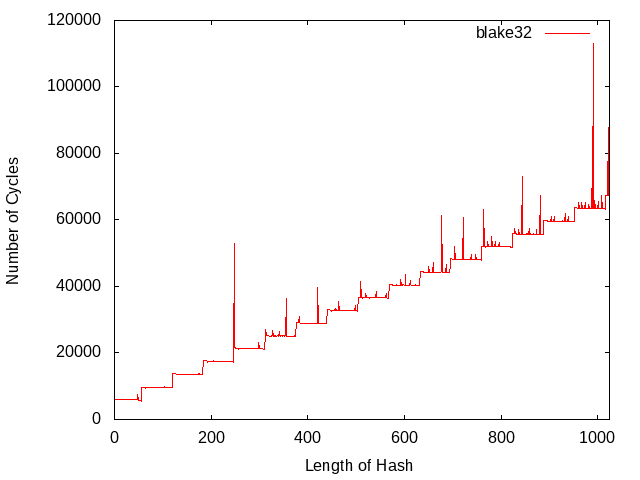
\includegraphics[scale=0.5]{images/blake32.png} 
        \caption{BLAKE with 32-bit words, 10 rounds, and 256-bit output}
    \end{center}
\end{figure}

From the graph above we see that there is a stepwise characteristic. The steps seem to increment every time the hash is divisible by 64. 
This characteristic is present due to the fact that during each iteration 2 words are taken from the message at one time. So a total of 64 bits
of the actual message is processed. This happens 8 times a round, therefore 512-bits are processed per round. So, as our hash size increases by 
multiples of 64 bytes we will see more and more iterations having to be processed.

\subsection{blake256}
    \begin{figure}[H]
        \begin{center}
            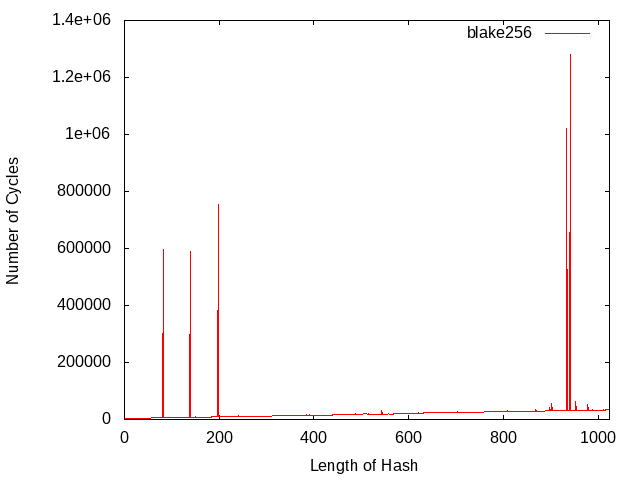
\includegraphics[scale=0.5]{images/blake256.png} 
            \caption{BLAKE with 32-bit words, 14 rounds, and 256-bit output}
        \end{center}
    \end{figure}

The graph above shows a very similar pattern to the blake32 graph. The reason is that blake256 also uses a 32 bit word size. The difference we
see between the blake32 and this graph is the number of cycles. When analyzing the data I found that the cycles per byte for blake32 was twice
that of blake256. This seems counter intuitive as blake256 has an additional 4 rounds to compute each iteration. I speculate that this is
due to the compiler options chosen by the script we ran to find the fastest implementation of each algorithm. The options chosen for blake256 were 
(compiler gcc -mcpu=arm1136jf-s -O -fomit-frame-pointer -fno-schedule-insns 4.4.5) versus the options for blake32 
(gcc -mcpu=arm9tdmi -O2 -fomit-frame-pointer 4.4.5). As we can see the architecture chosen by the script is not the target architecture and could
lead to a numer of mis-optimizations. 

\subsection{blake64}
    \begin{figure}[H]
        \begin{center}
            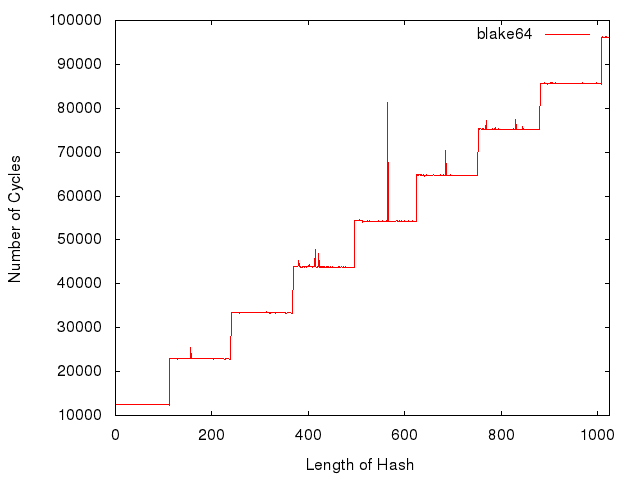
\includegraphics[scale=0.5]{images/blake64.png} 
            \caption{BLAKE with 64-bit words, 14 rounds, and 512-bit output }
        \end{center}
    \end{figure}

The blake64 hashing function increases the word size to 64 bits. Since nothing else changes we see that the widths of each step in our 
stepwise graph is doubled, so 1024 bits long. The cycles per byte were higher than that of the 32-bit word sizes. This is due to the 
fact that the target processor is a 32 bit architecture and does therefore doesn't have a chance to utilize 64 bit words. 

\subsection{blake512}
    \begin{figure}[H]
        \begin{center}
            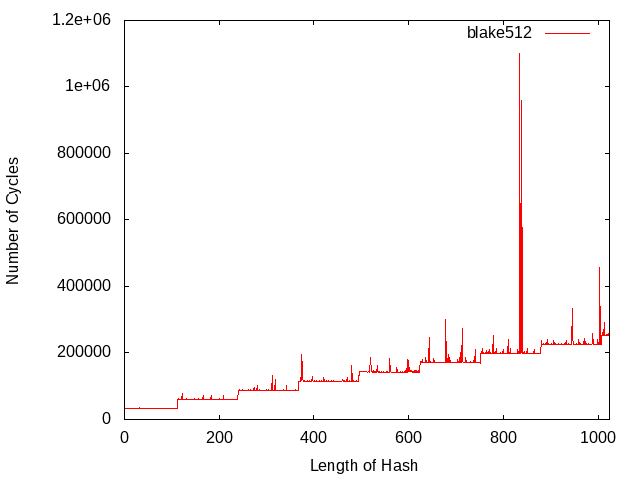
\includegraphics[scale=0.5]{images/blake512.png} 
            \caption{BLAKE with 64-bit words, 16 rounds, and 512-bit output}
        \end{center}
    \end{figure}
The difference between blake512 and blake64 is the number of rounds. This would explain the identical step width, 128 bytes, along with the increase
in cycles for blake512. 

\subsection{cubehash816}
I won't explain the details of cubehash here. I will instead talk about how the choice of variable sizes in the cube hash equation is reflected on the graph, along with the possible influence from the architecture. If we represent the equation as CubeHashi+r/b+f–h(m). Where i is the number of initialization rounds, r is the number of rounds per message block, b is the length of the blocks taken from the message, f is the number finalization rounds, h is the number of output bits, and m is the message. We're given that r is 8 rounds per block, b is 16 bytes in a block, and h is 512 bits of output.
    \begin{figure}[H]
        \begin{center}
            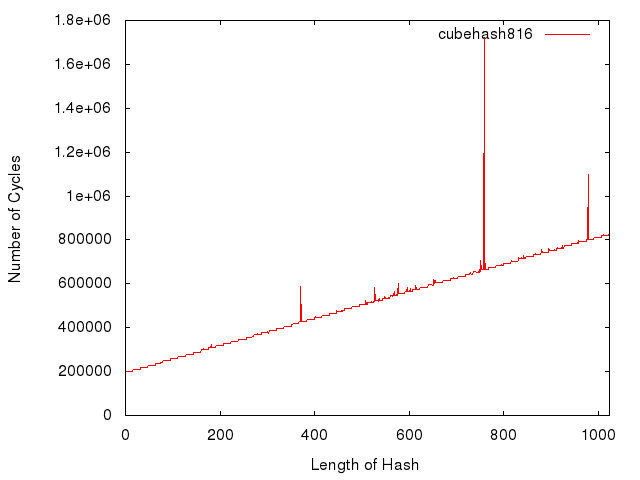
\includegraphics[scale=0.5]{images/cubehash816.png} 
            \caption{CubeHash8/16 with 512-bit output}
        \end{center}
    \end{figure}
It is a little hard to see in the above graph, but it takes on a similar shape to the graphs found in the blake algorithms. That is, it is as step like characteristics. The length of each step is 16 bytes, 128 bits. This appears to be from the size of the blocks processed each round. Each block is 16 bytes as described above. When the message increments by a multiple of 16 we see a rise in the step. As that's one more block that needs to be processed.  
Our target platform can provide 16, 32bit registers for the processing each block. This may be a responsible for the given speed.

\subsection{groestl256}
The groestl algorithm is another block cipher that is based from AES. This function works with l-bit blocks where l is 2n and n is the number of output bits. In this case n is 256 as denoted in the name. 
    \begin{figure}[H]
        \begin{center}
            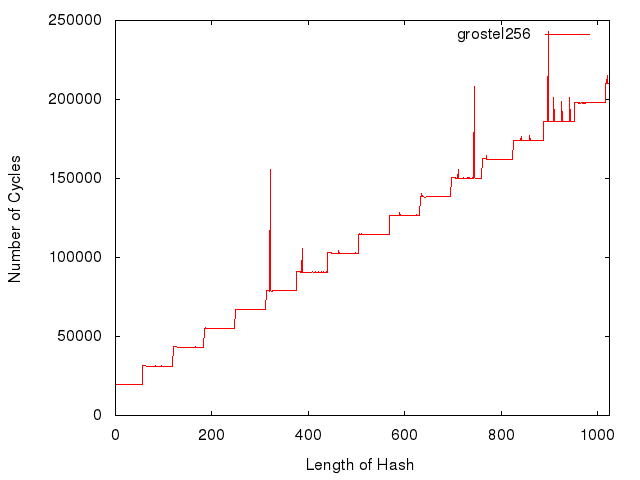
\includegraphics[scale=0.5]{images/grostel256.png} 
            \caption{Grøstl with 256-bit output}
        \end{center}
    \end{figure}
The graph above also shares the step like characteristics of the other graphs. Each step for this plot is 64 bytes, 512 bits in length. From what we know about groestl, it works with l-bit blocks, where we derived above l is 512 bits. We can then correlate this to the nature of the step size witnessed in the graph above.


\subsection{groestl512}
\subsection{jh224}
\subsection{keccak}
\subsection{keccakc1024}
\subsection{keccakc256}
\subsection{keccake448}
\subsection{keccake512}
\subsection{keccake768}
\subsection{md5}
\subsection{mgrastl256}
\subsection{sha256}
\subsection{sha512}
\subsection{skein10241024}
\subsection{skein256256}
\subsection{skein512256}
\subsection{skein512512}

% CONCLUSION   
%------------
% Contains:
%   - any overall conclusion we can draw from the results of ALL the graphs
%   - lessons learned
\section*{Conclusions}
\end{document}
